\documentclass[runningheads]{llncs}

\usepackage[T1]{fontenc}
\usepackage{graphicx}
\usepackage{amsmath,amssymb,mathtools}
\usepackage{booktabs,array,multirow}
\usepackage{xcolor}
\usepackage{enumitem}
\usepackage{listings}
\usepackage{hyperref}
\usepackage{tikz}
\usetikzlibrary{arrows.meta,positioning,shapes.geometric}
\usepackage{lineno}

%% ── note: llncs provides theorem, lemma, corollary, proposition,
%%   definition, remark, example, problem, and proof environments

%% ── math macros (Paper 1 — VHAGaR transfer mode) ────────────────────────────
\newcommand{\RR}{\mathbb{R}}
\newcommand{\NN}{\mathbb{N}}
\newcommand{\Ball}[2]{B_{#1}(#2)}
\newcommand{\conf}[3]{\mathcal{C}(#1,#2,#3)}   % 3-arg: network, input, class
\newcommand{\xp}{x'}
\newcommand{\ep}{\varepsilon}
\newcommand{\dD}{\delta_{\mathrm{diff}}}
\newcommand{\dO}{\delta_1}
\newcommand{\mI}{\mathcal{I}}
\newcommand{\up}{\mathrm{up}}
\newcommand{\dn}{\mathrm{dn}}
\newcommand{\Iup}{I^{\up}}
\newcommand{\Idn}{I^{\dn}}
\newcommand{\layer}[1]{^{[#1]}}
\newcommand{\net}[1]{^{\langle #1\rangle}}

%% ── math macros (Paper 2 — Formal analysis / counterexample) ────────────────
\newcommand{\R}{\mathbb{R}}           % alias for \RR used in Paper 2
\newcommand{\dN}[1]{\delta_1(N_{#1})}
\newcommand{\dNmod}[1]{\hat{\delta}_1(N_{#1})}
\newcommand{\ddiff}{\delta_{\mathrm{diff}}^{*}}
\newcommand{\ddiffmod}{\hat{\delta}_{\mathrm{diff}}}
\newcommand{\Xdom}{\mathcal{X}}
\newcommand{\Edom}{\mathcal{E}}
\newcommand{\Ffool}[1]{\mathcal{F}_{#1}}
\newcommand{\Fjoint}{\mathcal{F}_{1\wedge 2}}
% 2-class confidence shorthand (class fixed as c_tag; used in formal analysis)
\newcommand{\confB}[2]{\mathcal{C}(#1,#2)}

%% ── listing style ────────────────────────────────────────────────────────────
\lstset{basicstyle=\ttfamily\small,breaklines=true,
        keywordstyle=\color{blue!70!black},
        commentstyle=\color{gray},
        frame=single,framesep=3pt,numbers=left,numberstyle=\tiny\color{gray}}

\begin{document}

\title{Verification of Robustness Transfer Between Neural Networks}
\titlerunning{Verification of Robustness Transfer}

\author{Neta Nessing\inst{1} \and Shir Drive\inst{1} \and Dana Drachsler Cohen\inst{1}}
\authorrunning{N. Nessing et al.}

\institute{Technion, Israel\\
\email{\{neta.nessing,shir.drive,ddana\}@technion.ac.il}}

\maketitle

\begin{abstract}
Neural networks have achieved remarkable success across a wide range of applications, but they remain vulnerable to \emph{adversarial examples}---maliciously perturbed inputs designed to deceive the network. Verifying the robustness of neural networks against such attacks is a challenging task. In particular, verifying the \emph{global robustness} of a network---ensuring robustness for any input under a given perturbation function and scale---is computationally difficult.
In this work, we address the problem of \emph{robustness transfer verification}. Given a source network $N_1$ with a known robustness guarantee and a target network $N_2$, we compute a formal certificate guaranteeing $N_2$'s global robustness property. We encode this problem as a mixed-integer program (MIP).
Our approach supports seven perturbation types and employs four complementary tightening techniques: adversarial warm-starting, perturbation-difference interval propagation, inter-network interval bounds, and dependency analysis. We provide a complete formal analysis, including a proof that the transfer MIP yields a sound lower bound on the robustness improvement, a counterexample demonstrating that this bound can be strict, and a modified formulation that provides a matching upper bound over a restricted domain. Finally, we present a method for computing a sound upper bound during inference.

\keywords{Neural Network Verification \and Global Robustness \and Constrained Optimization}
\end{abstract}

\linenumbers

%% sections ───────────────────────────────────────────────────────────────────
%% ═══════════════════════════════════════════════════════════════════════════════
\section{Introduction}
\label{sec:intro}
%% ═══════════════════════════════════════════════════════════════════════════════

Deep neural networks are successful in various tasks but are also susceptible to adversarial examples: malicious input perturbations designed to deceive the network~\cite{szegedy2014,carlini2017,madry2018}. Many adversarial attacks target image classifiers and compute either an imperceptible change, bounded by a small $\varepsilon$ with respect to an $L_p$ norm, or a perceivable change obtained by perturbing a semantic feature of the input, such as brightness, translation, or occlusion.

A popular safety property for understanding a network's resilience to such attacks is \emph{local robustness}. Local robustness is parameterized by an input and its neighborhood: for a network classifier, the goal is to prove that the network classifies all inputs in the neighborhood the same. Several local robustness verifiers have been introduced for checking robustness in an $\varepsilon$-ball~\cite{singh2019,tjeng2019,wang2021}. However, local robustness is limited to reasoning about a single neighborhood at a time. To reason about a network's robustness over \emph{all} possible inputs, VHAGaR~\cite{vaghar} introduced the concept of \emph{global robustness}: computing the \emph{minimal globally robust bound}, the smallest confidence above which the network is provably robust to a given perturbation.

In practice, neural networks are rarely deployed in isolation. A common scenario involves training a more accurate network $N_2$ from an existing network $N_1$ via fine-tuning, distillation, or retraining. A natural question arises: \emph{does the robustness guarantee of $N_1$ transfer to $N_2$?} More precisely, if $N_1$ is known to be globally robust above some confidence threshold $\dN{1}$, can we certify $N_2$'s robustness without re-running the expensive global verification from scratch?

In this work, we address the problem of \emph{robustness transfer verification}. Given a source network $N_1$ and a target network $N_2$, we compute a confidence margin $\dD$ such that any input where $N_2$'s confidence exceeds $N_1$'s by more than $\dD$ inherits $N_1$'s robustness guarantee. Intuitively, $\dD$ captures the worst-case confidence gap between the two networks in the regime where $N_1$ is certifiably robust but $N_2$ can still be fooled. This problem is challenging for two main reasons. First, it requires encoding three forward passes --- $N_1(x)$, $N_2(x)$, and $N_2(\xp)$ --- simultaneously in a single optimization problem. Second, the perturbation introduces complex dependencies between the clean and perturbed computations that must be captured precisely for the resulting bounds to be tight.

We extend VHAGaR with a \emph{transfer mode} that encodes the robustness transfer problem as a mixed-integer program (MIP). Our MIP simultaneously models three forward passes --- $N_1(x)$, $N_2(x)$, and $N_2(\xp)$ --- linked by the perturbation constraint $\xp \in \mI_\ep(x)$. To make the resulting MIP tractable, we introduce four complementary tightening techniques: (1)~a \emph{hyper-adversarial attack} that provides a warm-start solution via projected gradient descent, (2)~\emph{perturbation-difference interval propagation} that bounds the activation differences between clean and perturbed passes, (3)~\emph{inter-network interval bounds} exploiting the structural similarity between $N_1$ and $N_2$, and (4)~\emph{dependency analysis} that identifies monotone relationships between activations. Our approach currently supports the $L_\infty$ perturbation and six semantic feature perturbations.

We provide a complete formal analysis of the transfer MIP's guarantees. We prove that the computed margin $\dD$ provides a \emph{sound lower bound}: $\dN{2} \geq \dN{1} + \dD$, meaning $N_2$'s global robustness bound is at least the sum of $N_1$'s bound and the transfer margin. We then exhibit a concrete counterexample with two simple linear networks demonstrating that the reverse inequality is \emph{false} in general --- the bound is strict. Finally, we propose a modified transfer MIP, replacing the constraint that $N_1$ is robust with the constraint that $N_1$ is \emph{foolable}, and prove that the resulting quantity $\ddiffmod$ satisfies the complementary upper bound $\dN{1} + \ddiffmod \geq \dNmod{2}$.

In summary, our main contributions are:
(1)~formalizing the robustness transfer problem and encoding it as a MIP with four tightening techniques (Section~\ref{sec:transfer}),
(2)~proving that the transfer MIP yields a sound lower bound on $N_2$'s robustness improvement over $N_1$ (Section~\ref{sec:formal}),
(3)~exhibiting an explicit counterexample showing the bound is strict, with a precise characterization of the gap (Section~\ref{sec:formal}), and
(4)~designing a modified formulation that provides a matching upper bound over the joint-foolable domain (Section~\ref{sec:formal}).

The rest of this paper is organized as follows. Section~\ref{sec:notation} provides background on network classifiers and formalizes the central quantities. Section~\ref{sec:perturbations} defines the supported perturbation models. Sections~\ref{sec:standard} and~\ref{sec:transfer} present the standard-mode and transfer-mode MIP formulations, respectively. Section~\ref{sec:modes} discusses the two attack constraint variants. Section~\ref{sec:formal} provides the full formal analysis. Section~\ref{sec:flags} describes the four tightening techniques. Section~\ref{sec:mip} gives the complete MIP formulation, and Sections~\ref{sec:inference} and~\ref{sec:conclusion} present the runtime inference procedure and conclusions.

%% ═══════════════════════════════════════════════════════════════════════════════
\section{Preliminaries}
\label{sec:notation}
%% ═══════════════════════════════════════════════════════════════════════════════

In this section, we provide background on neural network classifiers and formalize the central quantities used throughout this paper. We begin with the definitions of networks and confidence margins, then introduce the notions of robustness and foolability that underlie both the standard-mode and transfer-mode formulations.

\subsection{Neural Network Classifiers}

A classifier maps an input into a score vector over a set of labels (also called classes) $C$, i.e., it is a function $N : [0,1]^n \to \RR^{|C|}$. Given an input $x$, its classification is the label with the maximal score: $c = \mathrm{argmax}(N(x))$. We focus on classifiers implemented as neural networks. A neural network consists of an input layer followed by $L$ layers, where the last layer is the output layer. Layers consist of neurons, each connected to some or all neurons in the next layer.

We denote by $z_{m,k}$ the $k$-th neuron in layer $m$, for $m \in \{0, \ldots, L\}$ (where $0$ denotes the input layer) and $k \in \{1, \ldots, k_m\}$. The input layer $z_0$ passes the input $x$ to the next layer (i.e., $z_{0,k} = x_k$ for all $k \in [n]$). In a fully-connected layer, a neuron $z_{m,k}$ gets as input the outputs of all neurons in the preceding layer. It has a weight $w_{m,k,k'}$ for each input and a single bias $b_{m,k}$. Its function is the weighted sum of its inputs and bias followed by an activation function. Formally, the function of a non-input neuron is $z_{m,k} = \mathrm{ReLU}(\hat{z}_{m,k}) = \max(0, \hat{z}_{m,k})$, where $\hat{z}_{m,k}$ is the weighted sum: $\hat{z}_{m,k} = b_{m,k} + \sum_{k'=1}^{k_{m-1}} w_{m,k,k'} \cdot z_{m-1,k'}$. The network's parameters --- the weights and biases --- are determined by a training algorithm. The output layer consists of $|C|$ neurons, each outputting the score of one of the labels. We denote the output logits by $\hat{y}(x) = z^{[L]}(x)$.

Our definitions focus on fully-connected layers, but our implementation also supports convolutional layers and it is easily extensible to other layer types such as max-pooling layers~\cite{mipverify}.

\subsection{Confidence Margin}

The \emph{confidence margin} captures how certain a network is in its classification. Intuitively, a high confidence margin means the network assigns the correct class a score well above all other classes, making it harder for a perturbation to change the classification.

\begin{definition}[Confidence margin]
  \label{def:conf}
  Given a network $N$, an input $x$, and a class $c \in C$, the \emph{class confidence} of $N$ in $c$ at $x$ is:
  \[
    \conf{N}{x}{c} \;:=\; \hat{y}_c(x) \;-\; \max_{k \neq c}\, \hat{y}_k(x).
  \]
  The confidence $\conf{N}{x}{c} > 0$ if and only if $N$ classifies $x$ as $c$.

  \noindent\emph{Two-class setting.}
  When there are only two output classes $c_{\mathrm{tag}}$ and
  $c_{\mathrm{target}}$, we write $\confB{N}{x}$ as shorthand for
  $\conf{N}{x}{c_{\mathrm{tag}}} = \hat{y}_{c_{\mathrm{tag}}}(x)
  - \hat{y}_{c_{\mathrm{target}}}(x)$.
\end{definition}

\subsection{Robustness and Foolability}

We next define robustness and foolability with respect to a perturbation set. These notions form the building blocks of both the standard-mode and transfer-mode problems.

\begin{definition}[$(\varepsilon, c \to t)$-robustness]
  \label{def:robust}
  Given a network $N$ and a perturbation set $\mI_\ep(x)$ (defined per perturbation type in Section~\ref{sec:perturbations}), an input $x$ is \emph{$(\varepsilon, c \to t)$-robust} for $N$ if
  $\forall\, \xp \in \mI_\ep(x):\; N(\xp) \neq t$.
  That is, no perturbation in the allowed set causes $N$ to misclassify $x$ as the target class $t$.
\end{definition}

\begin{definition}[$N$-foolability]
  \label{def:foolable}
  An input $x\in\Xdom$ is \emph{$N$-foolable} if there exists a perturbation $\varepsilon\in\Edom$ with $x+\varepsilon\in\Xdom$ such that $\confB{N}{x+\varepsilon}\leq -\eta$, where $\eta > 0$ is a small attack margin (typically $10^{-3}$). We write $\Ffool{N}$ for the set of all $N$-foolable inputs.
\end{definition}

Intuitively, an input is foolable if the adversary can find a perturbation that causes the network to misclassify it. The set $\Ffool{N}$ contains all inputs that are vulnerable to adversarial attack under the given perturbation model.

\subsection{MIP Encoding of ReLU}

Our approach encodes the network's computation as a mixed-integer program (MIP). The JuMP/Gurobi MIP~\cite{jump,gurobi} encodes each linear layer exactly and linearizes every ReLU via the standard big-$M$ formulation with a binary variable $b \in \{0,1\}$:
\[
  a \;=\; \max(0,z), \qquad
  0 \le a \le M\,b, \qquad
  z \le a, \qquad
  a \le z + M(1-b).
\]
This encoding assigns each non-input ReLU neuron a binary variable, whose domain is $\{0,1\}$. Generally, the time complexity of a MIP problem over boolean and real variables is exponential in the number of boolean variables. To make the analysis more efficient, several works propose ways to identify boolean variables that can be removed (e.g., ReLUs whose inputs are non-positive or non-negative), thereby reducing the complexity~\cite{tjeng2019}.

\subsection{Formal Definitions of the Central Quantities}
\label{sec:notation:formal}

We now formalize the three central MIP quantities. Throughout, we use:
$\Xdom = [0,1]^n$ (input domain),
$\Edom = [-p,p]^n$ (perturbation ball for radius $p > 0$),
attack margin $\eta > 0$, and transition margin $\ep_0 > 0$ (both typically $10^{-3}$).

\begin{definition}[Standard-mode value]
  \label{def:delta1}
  The \emph{standard-mode value} of network $N_i$ is:
  \[
    \dN{i} \;:=\;
    \sup\bigl\{\,\confB{N_i}{x}
      \;\big|\;
      x\in\Ffool{i},\;
      \confB{N_i}{x}\geq 0
    \,\bigr\}.
  \]
  Intuitively, this is the maximum confidence $N_i$ attains on any input that is correctly classified yet can still be misclassified by some perturbation $\varepsilon\in\Edom$. Any input with confidence above $\dN{i}$ is provably robust.
\end{definition}

\begin{definition}[Transfer MIP --- original]
  \label{def:ddiff}
  Given networks $N_1$ and $N_2$ with pre-computed $\dN{1}$, the \emph{transfer value} is:
  \begin{align}
    \ddiff
    \;:=\;\sup\Bigl\{\,
      &\confB{N_2}{x}-\confB{N_1}{x}
      \;\Big|\notag\\
      &(\mathrm{C1})\;\confB{N_1}{x}\geq\dN{1}+\ep_0,\notag\\
      &(\mathrm{C2})\;\confB{N_2}{x}\geq\confB{N_1}{x},\notag\\
      &(\mathrm{C3})\;x\in\Ffool{2}
    \,\Bigr\}.\label{eq:ddiff}
  \end{align}
  Constraint C1 ensures $x$ lies in the region where $N_1$ is certifiably robust. C2 ensures $N_2$ is at least as confident as $N_1$. C3 ensures a perturbation exists that fools $N_2$. The objective maximizes the confidence gap, finding the worst-case scenario for the transfer guarantee.
\end{definition}

\begin{definition}[Modified transfer MIP]
  \label{def:ddiffmod}
  \begin{align}
    \ddiffmod
    \;:=\;\sup\Bigl\{\,
      &\confB{N_2}{x}-\confB{N_1}{x}
      \;\Big|\notag\\
      &(\widehat{\mathrm{C1}})\;x\in\Ffool{1},\notag\\
      &(\mathrm{C3})\;x\in\Ffool{2}
    \,\Bigr\}.\label{eq:ddiffmod}
  \end{align}
  The key change: C1 is replaced by $\widehat{\mathrm{C1}}$, which requires $x$ to be $N_1$-\emph{foolable} rather than $N_1$-robust.
\end{definition}

\begin{definition}[Joint-foolable set]
  \label{def:joint}
  $\Fjoint := \Ffool{1}\cap\Ffool{2}$: the set of inputs simultaneously foolable by both networks.
\end{definition}

\begin{definition}[Modified standard-mode value]
  \label{def:delta1mod}
  \[
    \dNmod{2} \;:=\;
    \sup\bigl\{\,\confB{N_2}{x}
      \;\big|\;
      x\in\Fjoint,\;
      \confB{N_2}{x}\geq 0
    \,\bigr\}.
  \]
  This is the maximum confidence $N_2$ achieves at inputs simultaneously foolable by \emph{both} networks. By definition, $\dNmod{2} \leq \dN{2}$, since restricting to the joint-foolable set can only decrease the supremum.
\end{definition}

%% ═══════════════════════════════════════════════════════════════════════════════
\section{Perturbation Models}
\label{sec:perturbations}
%% ═══════════════════════════════════════════════════════════════════════════════

In this section, we define the perturbation models supported by our framework. A perturbation is a function $f_P(x, \mathcal{E})$, defining how an input $x$ is perturbed given a perturbation amount specified by a vector $\mathcal{E}$. All perturbations are parameterized by a scalar $\ep > 0$ bounding their magnitude. For each perturbation type, we also define the \emph{perturbation-difference interval} $[\Idn, \Iup] \in \RR^n \times \RR^n$, which captures the element-wise range of $\xp - x$ at the input layer. These intervals are propagated layer-by-layer to tighten the MIP (Section~\ref{sec:flag:perturbed}).

\subsection{\texorpdfstring{$\ell_\infty$}{L-inf} Perturbation}

The $\ell_\infty$ perturbation has a perturbation limit $\ep \in [0,1]$ and is defined by a series of perturbations $\varepsilon_{i} \in [-\ep, \ep]$, for $i \in [n]$. The perturbation set is:
\[
  \mI_\ep(x) = \bigl\{\xp : \|\xp - x\|_\infty \le \ep,\;
  \xp \in [0,1]^n\bigr\}.
\]
In the MIP encoding, this translates to: $x_i - \ep \le x'_i \le x_i + \ep$ for every pixel $i$, with clipping to $[0,1]$.

The perturbation-difference interval is:
$\Idn_i = -\ep$, $\Iup_i = +\ep$ for all $i$.

\subsection{Brightness Perturbation}

Brightness is defined by a brightness level $e \in [0, \ep]$ such that $x'_i = x_i + e$ for all pixels $i$. The perturbation set is:
\[
  \mI_\ep(x) = \bigl\{\xp : \xp = x + e\,\mathbf{1},\; e \in [0, \ep]\bigr\}.
\]
In the MIP encoding, we add a scalar variable $e \in [0, \ep]$ and set $x'_i = x_i + e$.

Since $e \ge 0$, the brightness shift is non-negative. The perturbation-difference interval is therefore: $\Idn_i = 0$, $\Iup_i = +\ep$ for all $i$.

\subsection{Contrast Perturbation}

Contrast is defined by a scaling factor $e \in [1, 1+\ep]$ such that $x'_i = e \cdot x_i$. The perturbation set is:
\[
  \mI_\ep(x) = \bigl\{\xp : \xp = e\cdot x,\; e \in [1, 1+\ep]\bigr\}.
\]
In the MIP encoding, we add a scalar variable $e \in [1,1+\ep]$ and set $x'_i = e \cdot x_i$. Note that this introduces a bilinear constraint, which requires the Gurobi non-convex mode.

Since $e \ge 1$ and $x_i \ge 0$, we have $x'_i - x_i = (e-1)x_i \in [0, \ep]$. The perturbation-difference interval is an over-approximation: $\Idn_i = 0$, $\Iup_i = +\ep$ for all $i$.

\subsection{Translation Perturbation}

Translation is defined by shift coordinates $(d_h, d_w)$ with $|d_h|, |d_w| \le k$ pixels, and vacated positions are zero-padded. The shift direction is selected by binary variables $b_h, b_w \in \{0,1\}$ and offset variables $d_h, d_w \in [0,k]$.

Pixel values lie in $[0,1]$. After translation, the worst-case difference at any pixel is $\xp_i - x_i \in [-x_i, 1-x_i] \subseteq [-1, 1]$. We use the conservative perturbation-difference interval: $\Idn_i = -1$, $\Iup_i = +1$ for all $i$.

\subsection{Patch Perturbation}

A rectangular patch $P \subseteq [n]$ of pixels is perturbed by $\pm\ep$, while pixels outside $P$ are unchanged:
\[
  x'_i = x_i + e_i\,\ep, \quad e_i \in [-1, +1], \quad i \in P; \qquad
  x'_i = x_i, \quad i \notin P.
\]

The perturbation-difference interval reflects this structure:
\[
  \Idn_i = \begin{cases}-\ep & i \in P \\ 0 & i \notin P,\end{cases}
  \qquad
  \Iup_i = \begin{cases}+\ep & i \in P \\ 0 & i \notin P.\end{cases}
\]

\subsection{Occlusion Perturbation}

An occlusion perturbation sets a rectangular patch $P$ to zero, while pixels outside $P$ are unchanged:
\[
  x'_i = 0, \quad i \in P; \qquad x'_i = x_i, \quad i \notin P.
\]

Because $x_i \in [0,1]$ and $x'_i = 0$ inside $P$, the difference $x'_i - x_i = -x_i \in [-1, 0]$. Outside $P$, the difference is exactly zero. The perturbation-difference interval is therefore:
\[
  \Idn_i = \begin{cases}-1 & i \in P \\ 0 & i \notin P,\end{cases}
  \qquad
  \Iup_i = 0, \quad \forall\, i.
\]

\subsection{Summary}

Table~\ref{tab:perturbations} summarizes the perturbation sets and their corresponding input-layer difference intervals.

\begin{table}[ht]
  \centering
  \caption{Summary of perturbation sets and input-layer difference intervals.}
  \label{tab:perturbations}
  \begin{tabular}{llll}
    \toprule
    \textbf{Perturbation} & \textbf{Perturbation set} $\mI_\ep(x)$ &
    $\Idn_i$ & $\Iup_i$ \\
    \midrule
    $\ell_\infty$    & $\|\xp-x\|_\infty \le \ep$      & $-\ep$ & $+\ep$ \\
    Brightness       & $\xp = x + e$, $e\in[0,\ep]$    & $0$    & $+\ep$ \\
    Contrast         & $\xp = e\cdot x$, $e\in[1,1+\ep]$ & $0$ & $+\ep$ \\
    Translation      & pixel shift $\le k$ px, zero-pad & $-1$ & $+1$ \\
    Patch            & $\pm\ep$ inside patch $P$
                     & $-\ep \cdot \mathbf{1}_P$ & $+\ep \cdot \mathbf{1}_P$ \\
    Occlusion        & zero inside patch $P$
                     & $-\mathbf{1}_P$ & $0$ \\
    \bottomrule
  \end{tabular}
\end{table}

%% ═══════════════════════════════════════════════════════════════════════════════
\section{Standard Mode: Computing the Global Robustness Bound}
\label{sec:standard}
%% ═══════════════════════════════════════════════════════════════════════════════

In this section, we present the standard-mode formulation, which computes the global robustness bound for a single network. This bound serves as the foundation for the transfer-mode analysis in Section~\ref{sec:transfer}.

\subsection{Problem Definition}

We fix a source class $c$ and a target class $t$. The standard-mode MIP maximizes the confidence margin of the \emph{clean} input $x$ while requiring that a \emph{perturbed} input $\xp$ is misclassified as $t$:
\begin{equation}
  \label{eq:standard-obj}
  \dO \;=\; \max_{x,\,\xp}\; \conf{N_1}{x}{c}
  \quad \text{subject to} \quad
  \xp \in \mI_\ep(x),\quad
  \hat{y}_t(\xp) \ge \hat{y}_k(\xp)\;\forall k \neq t.
\end{equation}

Intuitively, the solution $\dO$ is the highest confidence at which the network can still be fooled. Any input classified with confidence above $\dO$ is provably robust: no perturbation in $\mI_\ep(x)$ can cause misclassification as $t$. This is equivalent to Definition~\ref{def:delta1}: $\dO = \dN{1}$ in the formal notation.

\subsection{MIP Encoding of the Confidence Margin}

The confidence margin involves $\max_{k \neq c} \hat{y}_k$, which is non-linear. We linearize it by introducing one binary variable $b_k \in \{0,1\}$ per class $k \neq c$, indicating whether class $k$ achieves the maximum:
\begin{align*}
  \delta &= \hat{y}_c - m, \\
  m &\ge \hat{y}_k \quad \forall\, k \neq c, \\
  m &\le \hat{y}_k + M(1 - b_k) \quad \forall\, k \neq c, \\
  \sum_{k \neq c} b_k &= 1,
\end{align*}
where $M$ is a sufficiently large constant. The solver then maximizes $\delta$. This encoding is exact: the binary variables ensure that $m$ equals the maximum logit among all non-$c$ classes, and the MIP objective finds the maximum confidence at which an adversarial perturbation exists.

%% ═══════════════════════════════════════════════════════════════════════════════
\section{Transfer Mode: Verifying Robustness Across Networks}
\label{sec:transfer}
%% ═══════════════════════════════════════════════════════════════════════════════

In this section, we present our main contribution: the transfer-mode formulation. We begin by motivating the problem, then describe our three-network MIP encoding, state the transfer MIP, and prove its correctness.

\subsection{Motivation}

Training a more accurate network $N_2$ from $N_1$ (e.g., via distillation or fine-tuning) often increases prediction confidence on correctly classified inputs. A natural question is: \emph{by how much can $N_2$'s confidence exceed $N_1$'s in the worst case, in the regime where $N_1$ is already certifiably robust but $N_2$ can still be fooled?} The answer to this question determines whether $N_1$'s robustness guarantee transfers to $N_2$.

\subsection{Three-Network Encoding}

To answer this question, the transfer mode encodes \textbf{three} forward passes simultaneously in a single MIP: $N_1(x)$, $N_2(x)$, and $N_2(\xp)$.

\begin{center}
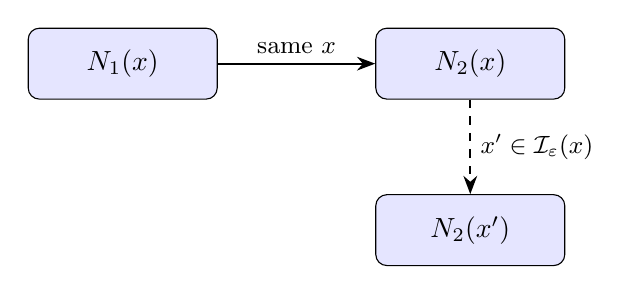
\begin{tikzpicture}[
  box/.style={draw,rounded corners,minimum width=2.4cm,minimum height=0.9cm,
               text centered,fill=blue!10},
  arr/.style={-Stealth,thick}]
  \node[box] (n1c) {$N_1(x)$};
  \node[box,right=2cm of n1c] (n2c) {$N_2(x)$};
  \node[box,below=1.2cm of n2c] (n2p) {$N_2(\xp)$};
  \draw[arr] (n1c) -- node[above,font=\small]{same $x$} (n2c);
  \draw[arr,dashed] (n2c) -- node[right,font=\small]{$\xp\in\mI_\ep(x)$} (n2p);
\end{tikzpicture}
\end{center}

Each forward pass uses a unique variable-name prefix to distinguish the three copies. The clean input $x$ is shared between $N_1(x)$ and $N_2(x)$, and the perturbed input $\xp$ is linked to $x$ via the perturbation constraint. Note that $N_1(\xp)$ is \emph{not} encoded: the transfer MIP only requires $N_1$'s confidence on the clean input to establish the robustness baseline, and $N_2$'s computation on both the clean and perturbed inputs to verify whether the attack succeeds. This saves all of the ReLU binary variables that would be needed for a fourth network pass, significantly reducing the problem size.

\subsection{Transfer MIP Formulation}

Let $c_1 = \conf{N_1}{x}{c}$, $c_2 = \conf{N_2}{x}{c}$, and $c_2' = \conf{N_2}{\xp}{c}$.
The transfer MIP is:

\begin{equation}
  \label{eq:transfer}
  \dD \;=\; \max_{x,\,\xp,\,e}\; (c_2 - c_1)
  \quad\text{s.t.}\quad
  \begin{cases}
    \xp \in \mI_\ep(x) & \text{(perturbation constraint)} \\
    c_1 \;\ge\; \dO + \epsilon_0 & \text{(T1: $N_1$ is certifiably robust)} \\
    c_2 - c_1 \;\ge\; 0 & \text{(T2: $N_2$ at least as confident as $N_1$)} \\
    \text{attack constraint on } N_2(\xp) & \text{(T3: $N_2$ can be fooled)}
  \end{cases}
\end{equation}

where $\epsilon_0 = 10^{-3}$ is a strict-inequality guard. In the formal notation of Section~\ref{sec:notation:formal}, this is exactly the transfer MIP of Definition~\ref{def:ddiff}, with $\dD = \ddiff$.

The constraint T1 restricts the search to inputs where $N_1$ is certifiably robust (its confidence exceeds the standard-mode bound $\dO$). Constraint T2 focuses on the regime where $N_2$ is more confident than $N_1$. Constraint T3 requires that a perturbation exists that fools $N_2$, making the transfer problem non-trivial. The encoding of T3 depends on the chosen attack mode (Section~\ref{sec:modes}).

\subsection{Correctness of the Transfer Guarantee}

We now prove that the transfer MIP provides a sound robustness certificate. The key insight is that any input violating the transfer guarantee would be a feasible solution to the MIP with objective value exceeding $\dD$, contradicting its optimality.

\begin{theorem}[Transfer Robustness]
  \label{thm:transfer}
  Let $\dO$ be the standard-mode value for $N_1$ on perturbation $(\ep, c \to t)$. Let $\dD$ be the optimal value of the transfer MIP~\eqref{eq:transfer}. Then for any input $x$:
  \[
    \conf{N_1}{x}{c} \;\ge\; \dO
    \;\;\text{and}\;\;
    \conf{N_2}{x}{c} - \conf{N_1}{x}{c} \;>\; \dD
    \;\;\implies\;\; x \text{ is } (\ep,c\to t)\text{-robust for } N_2.
  \]
\end{theorem}

\begin{proof}
  Suppose for contradiction that $x$ is \emph{not} $(\ep,c\to t)$-robust for $N_2$. Then there exists $\xp \in \mI_\ep(x)$ such that $N_2(\xp) = t$, meaning the attack constraint T3 holds.

  Since $\conf{N_1}{x}{c} \ge \dO$, constraint T1 is satisfied (with the $\epsilon_0$ guard). Since $\conf{N_2}{x}{c} - \conf{N_1}{x}{c} > \dD \geq 0$, constraint T2 is also satisfied.

  Therefore $(x, \xp)$ is a feasible solution to the transfer MIP~\eqref{eq:transfer} with objective value $c_2 - c_1 > \dD$, contradicting the fact that $\dD$ is the maximum feasible objective value.
\end{proof}

\begin{corollary}[Single-threshold inference]
  \label{cor:single}
  Define $\Delta := \dO + \dD$. If $\conf{N_1}{x}{c} \ge \dO$ and $\conf{N_2}{x}{c} > \Delta$, then $x$ is $(\ep, c \to t)$-robust for $N_2$.
\end{corollary}

This corollary shows that at inference time, the transfer guarantee reduces to checking two confidence thresholds, requiring only two forward passes and no additional optimization.

\begin{remark}
  Checking $\conf{N_2}{x}{c} > \Delta$ alone (without verifying $N_1$'s threshold) is \emph{unsound}: constraint T1 would not be guaranteed, making the transfer MIP potentially infeasible and $\dD$ meaningless. Both conditions must be verified.
\end{remark}

\subsection{Relationship to the Formal Quantities}

The transfer MIP~\eqref{eq:transfer} computes $\dD = \ddiff$, which satisfies $\dN{2} \geq \dN{1} + \ddiff$ (Theorem~\ref{thm:correct} in Section~\ref{sec:formal}). This is a \emph{lower bound}: knowing $\dD$ certifies that $N_2$'s standard-mode value is at least $\dO + \dD$, but $N_2$'s actual standard-mode value may be strictly larger. The precise gap and a counterexample are analyzed in Section~\ref{sec:formal}.

%% ═══════════════════════════════════════════════════════════════════════════════
\section{Attack Constraint Variants}
\label{sec:modes}
%% ═══════════════════════════════════════════════════════════════════════════════

In this section, we describe the two variants for encoding constraint T3 (``$N_2$ is fooled by $\xp$'') in the transfer MIP. The choice of variant determines whether the adversary targets a specific class or any misclassification.

\subsection{Targeted Attack}

In the targeted variant, the adversary forces $N_2$ to predict a specific target class $t$. Formally, the constraint requires:
\begin{equation}
  \label{eq:ctarget}
  \hat{y}_t\bigl(N_2(\xp)\bigr) \;\ge\; \hat{y}_k\bigl(N_2(\xp)\bigr)
  \quad \forall\, k \neq t,
\end{equation}
equivalently $\conf{N_2}{\xp}{t} \ge 0$. This is the more restrictive variant: the adversary must not only cause a misclassification but must steer the network toward a particular wrong class.

\subsection{Untargeted Attack}

In the untargeted variant, the adversary need only reduce $N_2$'s confidence in the true class $c$ to negative, causing any misclassification:
\begin{equation}
  \label{eq:ctag}
  \conf{N_2}{\xp}{c} \;\le\; 0.
\end{equation}

\subsection{Comparison}

Table~\ref{tab:modes} compares the two variants. The targeted variant has a smaller feasible region (the adversary must achieve a specific misclassification), leading to a larger or equal $\dD$ and thus a stronger transfer guarantee. The untargeted variant has a larger feasible region, yielding a smaller or equal $\dD$ and a weaker but more general guarantee.

\begin{table}[ht]
  \centering
  \caption{Comparison of targeted and untargeted attack constraints.}
  \label{tab:modes}
  \begin{tabular}{lll}
    \toprule
    \textbf{Property} & \textbf{Targeted} & \textbf{Untargeted} \\
    \midrule
    Attack type
      & $c \to t$ (specific class) & $c \to \text{any}$ \\
    Constraint on $N_2(\xp)$
      & $\hat{y}_t \ge \hat{y}_k,\;\forall k\neq t$
      & $\hat{y}_c < \hat{y}_k$ for some $k$ \\
    Feasible region    & Smaller (harder to satisfy) & Larger (easier) \\
    Resulting $\dD$    & Larger or equal & Smaller or equal \\
    Inference strength & Stronger guarantee & Weaker guarantee \\
    Typical use        & Specific adversary model & General robustness \\
    \bottomrule
  \end{tabular}
\end{table}


%% ═══════════════════════════════════════════════════════════════════════════════
\section{Formal Analysis}
\label{sec:formal}
%% ═══════════════════════════════════════════════════════════════════════════════

In this section, we provide a rigorous analysis of the relationship between the standard-mode values $\dN{1}$, $\dN{2}$, and the transfer quantity $\ddiff$. We prove that the transfer MIP provides a sound lower bound, exhibit a counterexample showing the bound is strict, analyze the root cause of the gap, and propose a modified formulation with a matching upper bound. Throughout this section, we use the two-class confidence $\confB{N}{x} = \hat{y}_{c_\mathrm{tag}}(x) - \hat{y}_{c_\mathrm{target}}(x)$ for compactness.

%% ────────────────────────────────────────────────────────────────────────────
\subsection{The Transfer MIP Provides a Lower Bound}
\label{sec:formal:correct}
%% ────────────────────────────────────────────────────────────────────────────

We first show that the transfer value $\ddiff$ provides a sound lower bound on the improvement in robustness from $N_1$ to $N_2$. Intuitively, any feasible point of the transfer MIP is also a feasible point of the standard-mode problem for $N_2$, so the transfer MIP explores a subset of the relevant search space.

\begin{theorem}[Lower bound on $\dN{2}$]
  \label{thm:correct}
  If the transfer MIP~\eqref{eq:ddiff} is feasible, then
  \[
    \boxed{\dN{2} \;\geq\; \dN{1} + \ddiff.}
  \]
\end{theorem}

\begin{proof}
  Fix $\epsilon>0$ and let $x^*$ be a nearly-optimal feasible point of~\eqref{eq:ddiff}, with $\varepsilon^*$ the corresponding attack perturbation (from C3). By feasibility:
  \begin{align}
    \confB{N_1}{x^*} &\geq \dN{1}+\ep_0, \tag{C1}\\
    \confB{N_2}{x^*} &\geq \confB{N_1}{x^*}, \tag{C2}\\
    x^* &\in\Ffool{2} \text{ via } \varepsilon^*, \tag{C3}\\
    \confB{N_2}{x^*}-\confB{N_1}{x^*} &\geq \ddiff-\epsilon. \tag{obj}
  \end{align}

  \textbf{Step 1.} We lower-bound $\confB{N_2}{x^*}$:
  \begin{align*}
    \confB{N_2}{x^*}
    &= \confB{N_1}{x^*}+\bigl(\confB{N_2}{x^*}-\confB{N_1}{x^*}\bigr)\\
    &\geq (\dN{1}+\ep_0)+(\ddiff-\epsilon)
    \geq \dN{1}+\ddiff-\epsilon.
  \end{align*}

  \textbf{Step 2.} We show $x^*$ is feasible for the standard-mode MIP on $N_2$. By C2 and C1, $\confB{N_2}{x^*}\geq\confB{N_1}{x^*}\geq\dN{1}+\ep_0>0$, so $N_2$ correctly classifies $x^*$. Combined with C3 ($x^*\in\Ffool{2}$), the pair $(x^*,\varepsilon^*)$ is feasible for the standard-mode MIP on $N_2$. Hence:
  \[
    \dN{2} \;\geq\;\confB{N_2}{x^*} \;\geq\;\dN{1}+\ddiff-\epsilon.
  \]
  Since $\epsilon>0$ is arbitrary, we conclude $\dN{2}\geq\dN{1}+\ddiff$.
\end{proof}

\begin{remark}[The gap is always positive]
  \label{rem:gap}
  Let $x^*$ achieve the supremum in~\eqref{eq:ddiff}. The proof shows:
  \[
    \dN{2} - (\dN{1}+\ddiff)
    \;\geq\;
    \confB{N_1}{x^*}-\dN{1}
    \;\geq\;\ep_0\;>\;0.
  \]
  The gap is always positive because constraint C1 forces $\confB{N_1}{x^*}>\dN{1}$. This surplus $\confB{N_1}{x^*}-\dN{1}$ is the precise ``slack'' that makes the theorem strict.
\end{remark}

%% ────────────────────────────────────────────────────────────────────────────
\subsection{The Reverse Inequality Fails: A Counterexample}
\label{sec:formal:counter}
%% ────────────────────────────────────────────────────────────────────────────

We next show that the reverse inequality, $\dN{1}+\ddiff \geq \dN{2}$, is false in general. We exhibit two explicit linear networks that produce a strict gap.

\subsubsection{Network Definitions}

We consider two linear networks over $\Xdom=[0,1]^2$, with perturbation radius $p=0.1$, and margins $\eta=\ep_0=10^{-3}$.

\medskip
\begin{center}
\begin{tabular}{lll}
\toprule
Network & Logits & Confidence margin $\confB{N}{\cdot}$ \\
\midrule
$N_1$ & $[x_1,\ x_2]$ & $x_1-x_2$ \\[4pt]
$N_2$ & $[2x_1,\ 5x_2]$ & $2x_1-5x_2$ \\
\bottomrule
\end{tabular}
\end{center}

\medskip\noindent
Both are two-layer networks: an identity first layer, an inactive ReLU (since $x_1,x_2\geq 0$), and a diagonal second layer ($\mathrm{diag}(1,1)$ for $N_1$, $\mathrm{diag}(2,5)$ for $N_2$). Despite their simplicity, these networks suffice to demonstrate that the gap can be substantial.

\subsubsection{Foolability Conditions}

We derive the foolability conditions for each network.

$N_1$ is fooled at $x+\varepsilon$ if and only if $(x_2+\varepsilon_2)-(x_1+\varepsilon_1)\geq\eta$, i.e., $\varepsilon_2-\varepsilon_1\geq(x_1-x_2)+\eta$. The maximum of $\varepsilon_2-\varepsilon_1$ over $\Edom$ is $2p=0.2$, so:
\[
  x\in\Ffool{1}
  \;\Longleftrightarrow\;
  x_1-x_2\;\leq\;2p-\eta\;=\;0.199.
\]

$N_2$ is fooled at $x+\varepsilon$ if and only if $5(x_2+\varepsilon_2)-2(x_1+\varepsilon_1)\geq\eta$, i.e., $5\varepsilon_2-2\varepsilon_1\geq(2x_1-5x_2)+\eta$. The maximum of $5\varepsilon_2-2\varepsilon_1$ over $\Edom$ is $5p+2p=0.7$, so:
\[
  x\in\Ffool{2}
  \;\Longleftrightarrow\;
  2x_1-5x_2\;\leq\;5p+2p-\eta\;=\;0.699.
\]

\subsubsection{Computing the Quantities}

We now compute $\dN{1}$, $\dN{2}$, and $\ddiff$ for our counterexample networks.

\emph{Standard-mode value $\dN{1}$.} We maximize $x_1-x_2$ subject to $x_1-x_2\leq 0.199$ and $x\in[0,1]^2$: $\dN{1}=0.199$, achieved at $x^{(1)}=(1,\,0.801)$.

\emph{Standard-mode value $\dN{2}$.} We maximize $2x_1-5x_2$ subject to $2x_1-5x_2\leq 0.699$ and $x\in[0,1]^2$: $\dN{2}=0.699$, achieved at $x^{(2)}=(1,\,0.2602)$ with attack $\varepsilon^*=(-0.1,+0.1)$.

\emph{Transfer value $\ddiff$.} The objective is $\confB{N_2}{x}-\confB{N_1}{x}=(2x_1-5x_2)-(x_1-x_2)=x_1-4x_2$. The constraints are:
\begin{align*}
  \mathrm{C1}:&\quad x_1-x_2\geq 0.200,\\
  \mathrm{C2}:&\quad x_1-4x_2\geq 0,\\
  \mathrm{C3}:&\quad 2x_1-5x_2\leq 0.699.
\end{align*}
Setting $x_2=0$ (which minimizes the $-4x_2$ penalty), C1 gives $x_1\geq 0.200$ and C3 gives $x_1\leq 0.3495$. Maximizing $x_1$ yields:
\[
  x^*=(0.3495,\,0),
  \qquad
  \ddiff=x_1^*-4\cdot 0=\mathbf{0.3495}.
\]

Note that $\confB{N_1}{x^*}=0.3495$, which is substantially larger than $\dN{1}=0.199$. This is the source of the gap.

\subsubsection{The Counterexample}

\begin{center}
\renewcommand{\arraystretch}{1.5}
\begin{tabular}{lc}
\toprule
Quantity & Value \\
\midrule
$\dN{1}$ & $0.199$ \\
$\ddiff$ & $0.3495$ \\
$\dN{1}+\ddiff$ & $\mathbf{0.5485}$ \\
\midrule
$\dN{2}$ & $\mathbf{0.699}$ \\
\midrule
Gap: $\dN{2}-(\dN{1}+\ddiff)$ & $\mathbf{0.1505}$ \\
\bottomrule
\end{tabular}
\end{center}

\[
  \dN{1}+\ddiff \;=\; 0.5485 \;\;\mathbf{<}\;\; 0.699 \;=\; \dN{2}.
\]

The gap equals exactly $\confB{N_1}{x^*}-\dN{1}=0.3495-0.199=0.1505$, consistent with Remark~\ref{rem:gap}.

%% ────────────────────────────────────────────────────────────────────────────
\subsection{Root-Cause Analysis}
\label{sec:formal:analysis}
%% ────────────────────────────────────────────────────────────────────────────

Theorem~\ref{thm:correct} and the counterexample together establish that $\dN{1}+\ddiff$ is a \emph{strict lower bound} on $\dN{2}$, with gap:
\[
  \mathrm{gap}
  \;=\;
  \underbrace{\confB{N_1}{x^*}}_{\geq\,\dN{1}+\ep_0\;(\mathrm{C1})}
  -\;
  \dN{1}
  \;\geq\;\ep_0\;>\;0.
\]

The structural reason is the following. The transfer MIP searches for an $x^*$ that simultaneously satisfies C1 (high $N_1$-confidence) and C3 ($N_2$-foolable). Because $N_1$ and $N_2$ have \emph{different} decision boundaries, the $N_2$-foolable region can contain points with $N_1$-confidence far above $\dN{1}$. At such an $x^*$, the quantity $\confB{N_2}{x^*}=\confB{N_1}{x^*}+\ddiff$ is large, but the formula $\dN{1}+\ddiff$ loses the surplus $\confB{N_1}{x^*}-\dN{1}$.

Equivalently, the transfer MIP's feasible set $\{x:\mathrm{C1{+}C3}\}$ is a \emph{proper subset} of the standard-mode feasible set for $N_2$ ($\{x\in\Ffool{2}\}$):
\[
  \dN{2}
  \;=\;
  \sup_{x\in\Ffool{2}}\confB{N_2}{x}
  \;\geq\;
  \sup_{x:\,\mathrm{C1{+}C3}}\confB{N_2}{x}
  \;\geq\;
  \sup_{x:\,\mathrm{C1{+}C2{+}C3}}\bigl[\confB{N_1}{x}+\ddiff\bigr]
  \;\geq\;
  \dN{1}+\ddiff.
\]
The first inequality can be strict because $\Ffool{2}$ contains points with high $\confB{N_2}{\cdot}$ that \emph{violate} C1 (i.e., they are not $N_1$-robust).

%% ────────────────────────────────────────────────────────────────────────────
\subsection{A Modified Formulation with a Matching Upper Bound}
\label{sec:formal:modified}
%% ────────────────────────────────────────────────────────────────────────────

\subsubsection{Motivation}

Remark~\ref{rem:gap} reveals that the gap is driven by C1 forcing $\confB{N_1}{x^*}>\dN{1}$. To close the gap, we replace C1 with its logical opposite: instead of requiring $N_1$ to be \emph{robust} at $x$, we require $N_1$ to be \emph{foolable} at $x$. This simultaneously restricts the standard-mode problem for $N_2$ to the same joint-foolability region.

The modified transfer MIP is Definition~\ref{def:ddiffmod}, with modified standard-mode value $\dNmod{2}$ (Definition~\ref{def:delta1mod}). Note that $\dNmod{2}\leq\dN{2}$ by definition: restricting to $\Fjoint\subseteq\Ffool{2}$ can only decrease the supremum. The gap $\dN{2}-\dNmod{2}$ measures the advantage $N_2$ has at points where it is foolable but $N_1$ is not --- the ``exclusive vulnerability'' of $N_2$.

\subsubsection{MIP Encoding}

The constraint $\widehat{\mathrm{C1}}$ introduces a second perturbation variable $\varepsilon^{(1)}\in\Edom$ with the foolability constraint $\confB{N_1}{x+\varepsilon^{(1)}}\leq-\eta$, encoded exactly as in the standard-mode MIP for $N_1$. Constraint C3 is encoded as before. The resulting program has $O(|N_1|+|N_2|)$ binary variables and is solvable by standard MIP solvers.

\subsubsection{Main Result}

\begin{theorem}[Upper bound on the joint standard-mode value]
  \label{thm:modified}
  \[
    \boxed{\dN{1} + \ddiffmod \;\geq\; \dNmod{2}.}
  \]
\end{theorem}

\begin{proof}
  Fix $\epsilon>0$ and let $x^{**}$ be a nearly-optimal feasible point of $\dNmod{2}$ (Definition~\ref{def:delta1mod}), i.e., $x^{**}\in\Fjoint$, $\confB{N_2}{x^{**}}\geq 0$, $\confB{N_2}{x^{**}}\geq\dNmod{2}-\epsilon$.

  \textbf{Step 1.} Since $x^{**}\in\Ffool{1}$, by Definition~\ref{def:delta1}, $\confB{N_1}{x^{**}}\leq\dN{1}$.

  \textbf{Step 2.} Since $x^{**}\in\Ffool{1}$ satisfies $\widehat{\mathrm{C1}}$ and $x^{**}\in\Ffool{2}$ satisfies C3, $x^{**}$ is feasible for~\eqref{eq:ddiffmod}. Hence: $\ddiffmod \;\geq\; \confB{N_2}{x^{**}}-\confB{N_1}{x^{**}}$.

  \textbf{Step 3.} Combining:
  \begin{align*}
    \dN{1}+\ddiffmod
    &\geq\dN{1}+\confB{N_2}{x^{**}}-\confB{N_1}{x^{**}}\\
    &\geq\confB{N_1}{x^{**}}+\confB{N_2}{x^{**}}-\confB{N_1}{x^{**}}
    \quad\text{(Step 1: $\dN{1}\geq\confB{N_1}{x^{**}}$)}\\
    &=\confB{N_2}{x^{**}} \;\geq\;\dNmod{2}-\epsilon.
  \end{align*}
  Since $\epsilon>0$ is arbitrary, $\dN{1}+\ddiffmod\geq\dNmod{2}$.
\end{proof}

\begin{corollary}[Sandwich bounds]
  \label{cor:sandwich}
  If both transfer MIPs are feasible:
  \[
    \dN{1}+\ddiff
    \;\leq\;
    \dN{2},
    \qquad\qquad
    \dN{1}+\ddiffmod
    \;\geq\;
    \dNmod{2}.
  \]
\end{corollary}

\begin{remark}[Complementary regions]
  The two transfer quantities explore complementary regions: the original $\ddiff$ searches over $N_1$-\emph{robust} $\cap$ $N_2$-\emph{foolable} inputs, while $\ddiffmod$ searches over $N_1$-\emph{foolable} $\cap$ $N_2$-\emph{foolable} inputs. These regions are disjoint. In particular, $\ddiffmod$ can be negative (if $N_1$ always has higher confidence than $N_2$ in $\Fjoint$), while $\ddiff \geq 0$ by constraint C2.
\end{remark}

%% ────────────────────────────────────────────────────────────────────────────
\subsection{Numerical Verification}
\label{sec:formal:numerical}
%% ────────────────────────────────────────────────────────────────────────────

We verify Theorem~\ref{thm:modified} on the counterexample networks from Section~\ref{sec:formal:counter}.

\emph{Modified transfer value $\ddiffmod$.} We maximize $x_1-4x_2$ subject to $x_1-x_2\leq 0.199$ ($N_1$-foolable) and $2x_1-5x_2\leq 0.699$ ($N_2$-foolable), with $x\in[0,1]^2$. Setting $x_2=0$: $x_1\leq\min(0.199,\,0.3495)=0.199$. This yields $\ddiffmod = \mathbf{0.199}$.

\emph{Modified standard-mode value $\dNmod{2}$.} We maximize $2x_1-5x_2$ subject to both foolability constraints. At $x_2=0$: $x_1\leq 0.199$, so $\dNmod{2}=2\times 0.199=\mathbf{0.398}$.

\begin{center}
\renewcommand{\arraystretch}{1.5}
\begin{tabular}{lc}
\toprule
Quantity & Value \\
\midrule
$\dN{1}$ & $0.199$ \\
$\ddiffmod$ & $0.199$ \\
$\dN{1}+\ddiffmod$ & $\mathbf{0.398}$ \\
\midrule
$\dNmod{2}$ & $\mathbf{0.398}$ \\
\midrule
$\dN{1}+\ddiffmod\geq\dNmod{2}$? & \textbf{YES} (equality holds) \\
\midrule\midrule
$\dN{2}$ (unrestricted) & $0.699$ \\
Joint gap: $\dN{2}-\dNmod{2}$ & $0.301$ \\
\bottomrule
\end{tabular}
\end{center}

Equality holds in Theorem~\ref{thm:modified} because the binding constraint is simultaneously $\widehat{\mathrm{C1}}$ and C3, making $x^{**}$ the argmax for both $\dNmod{2}$ and $\ddiffmod$. The joint gap of $0.301$ reflects $N_2$'s foolable region that is $N_1$-robust --- precisely the regime probed by the original transfer MIP.

%% ────────────────────────────────────────────────────────────────────────────
\subsection{Discussion: Two Complementary Formulations}
\label{sec:formal:discussion}
%% ────────────────────────────────────────────────────────────────────────────

The original and modified transfer MIPs provide complementary views of the robustness relationship between two networks. Table~\ref{tab:complementary} summarizes their characteristics.

\begin{table}[ht]
\centering
\caption{Comparison of the two transfer MIP formulations.}
\label{tab:complementary}
\renewcommand{\arraystretch}{1.3}
\begin{tabular}{lll}
\toprule
\textbf{Formulation} & \textbf{Feasible region} & \textbf{Bound direction} \\
\midrule
Original $\ddiff$ & $N_1$-robust $\cap$ $N_2$-foolable
  & $\dN{2}\geq\dN{1}+\ddiff$ (lower bound) \\
Modified $\ddiffmod$ & $N_1$-foolable $\cap$ $N_2$-foolable
  & $\dN{1}+\ddiffmod\geq\dNmod{2}$ (upper bound) \\
\bottomrule
\end{tabular}
\end{table}

The original formulation asks: ``By how much can $N_2$'s confidence exceed $N_1$'s, at a point where $N_1$ is provably robust?'' Theorem~\ref{thm:correct} shows this provides a lower bound on $\dN{2}-\dN{1}$.

The modified formulation asks: ``At points hardest for \emph{both} networks simultaneously, how much more confident is $N_2$ than $N_1$?'' Theorem~\ref{thm:modified} shows this provides an upper bound on $\dNmod{2}-\dN{1}$.

Together, the two quantities bracket the robustness difference from both sides over their respective domains.

%% ═══════════════════════════════════════════════════════════════════════════════
\section{Tightening Techniques}
\label{sec:flags}
%% ═══════════════════════════════════════════════════════════════════════════════

In this section, we present four complementary techniques for tightening the MIP relaxation. As described in Section~\ref{sec:standard}, the time complexity of the MIP is governed by the number of boolean variables. To enable the MIP solver to reach a solution efficiently, we introduce techniques that reduce the search space by providing tighter bounds and warm-start solutions. The four techniques can be combined freely, progressively trading preprocessing time for faster solver convergence.

\begin{table}[ht]
  \centering
  \caption{Overview of the four tightening techniques.}
  \label{tab:flags}
  \begin{tabular}{llll}
    \toprule
    \textbf{Technique} & \textbf{Method} & \textbf{Preprocess} & \textbf{Benefit} \\
    \midrule
    Hyper-adversarial attack
      & PGD warm-start   & Python PGD & Incumbent cutoff \\
    Perturbation-diff.\ intervals
      & Interval propagation & Interval arith. & Activation bounds \\
    Inter-network intervals
      & Weight-difference bounds & Interval arith. & Cross-network bounds \\
    Dependency analysis
      & Monotonicity signatures & Symbolic prop. & Ordering constraints \\
    \bottomrule
  \end{tabular}
\end{table}

%% ─────────────────────────────────────────────────────────────────────────────
\subsection{Hyper-Adversarial Attack}
\label{sec:flag:hyper}
%% ─────────────────────────────────────────────────────────────────────────────

Our first technique expedites the tightening of the lower bound by efficiently computing a suboptimal feasible solution and providing it to the MIP solver. Before launching the MIP solver, we run a projected gradient descent (PGD) attack~\cite{madry2018} to find a feasible solution $(x^\star, \xp{}^\star)$ with objective value $v^\star$.

This solution is used in two ways. First, as an \emph{incumbent cutoff}: the solver can prune any branch whose objective value cannot exceed $v^\star$. Formally, we set the Gurobi incumbent to $v^\star$, enabling the solver to discard large portions of the search tree.

Second, as a \emph{binary warm-start}: for each ReLU binary variable $b_j$, we compute the activation sign at the PGD solution and provide it as a hint:
\[
  b_j^{\text{hint}} \;=\; \mathbf{1}\!\left[z^{[l]}_j(x^\star) \ge 0\right].
\]
These hints guide the solver toward the optimal branching decisions, significantly reducing the number of explored nodes.

%% ─────────────────────────────────────────────────────────────────────────────
\subsection{Perturbation-Difference Interval Propagation}
\label{sec:flag:perturbed}
%% ─────────────────────────────────────────────────────────────────────────────

Our second technique bounds the activation differences between the clean and perturbed forward passes. For each layer $l$, we compute an interval $[\Idn\layer{l}, \Iup\layer{l}]$ bounding the element-wise difference $a\net{pert}\layer{l} - a\net{org}\layer{l}$. The same propagation applies to both the $N_1$ and $N_2$ network pairs.

\emph{Initialization (input layer).} From Table~\ref{tab:perturbations}:
$\Idn\layer{0} = \Idn$, $\Iup\layer{0} = \Iup$.

\emph{Linear layer propagation.} For weight matrix $W\layer{l}$ (the bias cancels in the difference):
\begin{align}
  \Iup\layer{l} &= (W\layer{l})^+ \,\Iup\layer{l-1}
                  + (W\layer{l})^- \,\Idn\layer{l-1}, \label{eq:Iup-lin} \\
  \Idn\layer{l} &= (W\layer{l})^+ \,\Idn\layer{l-1}
                  + (W\layer{l})^- \,\Iup\layer{l-1}, \label{eq:Idn-lin}
\end{align}
where $W^+ = \max(W,0)$ and $W^- = \min(W,0)$.

\emph{ReLU layer propagation.} We use a linear over-approximation:
\[
  \Iup\layer{l} \;\leftarrow\; \max\!\bigl(0,\, \Iup\layer{l-1}\bigr),
  \qquad
  \Idn\layer{l} \;\leftarrow\; \min\!\bigl(0,\, \Idn\layer{l-1}\bigr).
\]

\emph{Added MIP constraints.} At every layer $l$ and neuron $j$:
\begin{equation}
  \label{eq:perturbed-constraints}
  a\net{org}\layer{l}_j + \Idn\layer{l}_j
  \;\le\; a\net{pert}\layer{l}_j
  \;\le\; a\net{org}\layer{l}_j + \Iup\layer{l}_j.
\end{equation}
These constraints couple the clean and perturbed forward passes, tightening the LP relaxation. We next prove their soundness.

\emph{Soundness, completeness, and tightness.} We distinguish three properties of added constraints in a MIP verifier:
\begin{itemize}
  \item \textbf{Soundness} (no false negatives): a constraint is sound if it is satisfied by every feasible point of the original MIP, so it never removes a real solution.
  \item \textbf{Completeness} (no false positives): a constraint is complete if it does not introduce spurious feasible points, so the LP relaxation does not admit solutions that could not arise from any true $(x,\xp)$ pair.
  \item \textbf{Tightness} (quality of approximation): a sound constraint is tight at a point if the bound it provides equals the true value there.
\end{itemize}

The interval constraints~\eqref{eq:perturbed-constraints} are \textbf{sound and complete but not always tight}. They are sound because the propagated intervals are genuine over-approximations (Theorem~\ref{thm:pert-sound}). They are complete because, being over-approximations, they can only widen the set of allowed activations. They are not always tight because the ReLU propagation step uses a linear over-approximation that is loose when one of the two compared activations is negative and the other is positive.

\begin{theorem}[Soundness of perturbation-difference interval propagation]
  \label{thm:pert-sound}
  Let $N$ be a ReLU network with weights $W\layer{l}$, biases $b\layer{l}$. Fix any $x$ and $\xp$ such that $\xp_i - x_i \in [\Idn_i\layer{0},\, \Iup_i\layer{0}]$ elementwise. Then for every layer $l$ and every neuron $j$:
  \[
    a_j\layer{l}(\xp) - a_j\layer{l}(x)
    \;\in\;
    \bigl[\Idn_j\layer{l},\; \Iup_j\layer{l}\bigr],
  \]
  where $[\Idn\layer{l}, \Iup\layer{l}]$ are computed by the recursion in~\eqref{eq:Iup-lin}--\eqref{eq:Idn-lin} and the ReLU propagation step.
\end{theorem}

\begin{proof}
  By induction on $l$.

  \textbf{Base case} ($l = 0$): $a\layer{0}(x) = x$ and $a\layer{0}(\xp) = \xp$, so $a_i\layer{0}(\xp) - a_i\layer{0}(x) = \xp_i - x_i \in [\Idn_i\layer{0}, \Iup_i\layer{0}]$ by assumption.

  \textbf{Inductive step --- linear layer.} Assume $\Delta_i := a_i\layer{l-1}(\xp) - a_i\layer{l-1}(x) \in [\Idn_i\layer{l-1}, \Iup_i\layer{l-1}]$ for all $i$. The pre-activation difference at neuron $j$ is $z_j\layer{l}(\xp) - z_j\layer{l}(x) = \sum_i W_{ji}\layer{l}\, \Delta_i$. Decompose $W_{ji}\layer{l} = W_{ji}^+ + W_{ji}^-$ with $W_{ji}^+ \ge 0$, $W_{ji}^- \le 0$. Then:
  \begin{align*}
    z_j\layer{l}(\xp) - z_j\layer{l}(x)
    &\;\le\; \sum_i W_{ji}^+\, \Iup_i\layer{l-1}
             + \sum_i W_{ji}^-\, \Idn_i\layer{l-1}
    \;=\; \Iup_j\layer{l}, \\
    z_j\layer{l}(\xp) - z_j\layer{l}(x)
    &\;\ge\; \sum_i W_{ji}^+\, \Idn_i\layer{l-1}
             + \sum_i W_{ji}^-\, \Iup_i\layer{l-1}
    \;=\; \Idn_j\layer{l},
  \end{align*}
  using monotonicity of multiplication by a non-negative (resp.\ non-positive) scalar. The bias cancels in the difference.

  \textbf{Inductive step --- ReLU layer.} Write $\Delta_j^z := z_j\layer{l}(\xp) - z_j\layer{l}(x) \in [\Idn_j\layer{l}, \Iup_j\layer{l}]$. For any $u, v \in \RR$: $\max(0,u) - \max(0,v) \le \max(0, u - v)$ and $\max(0,u) - \max(0,v) \ge \min(0, u - v)$. Applying with $u = z_j(\xp)$, $v = z_j(x)$:
  \[
    \min(0, \Delta_j^z) \;\le\;
    a_j\layer{l}(\xp) - a_j\layer{l}(x)
    \;\le\; \max(0, \Delta_j^z).
  \]
  Since $\Delta_j^z \le \Iup_j\layer{l}$, we have $\max(0, \Delta_j^z) \le \max(0, \Iup_j\layer{l})$, and since $\Delta_j^z \ge \Idn_j\layer{l}$, we have $\min(0, \Delta_j^z) \ge \min(0, \Idn_j\layer{l})$. The updated interval $[\min(0,\Idn_j\layer{l}),\, \max(0,\Iup_j\layer{l})]$ is exactly what the ReLU propagation step produces.
\end{proof}

\begin{corollary}[Constraint validity]
  Every feasible point $(x, \xp, \{a\net{m}\layer{l}\})$ of the MIP already satisfies constraints~\eqref{eq:perturbed-constraints}. Adding them therefore does not cut off any feasible solution, but shrinks the LP relaxation polytope, strengthening the dual bound and reducing branch-and-bound effort.
\end{corollary}

%% ─────────────────────────────────────────────────────────────────────────────
\subsection{Inter-Network Interval Bounds}
\label{sec:flag:intervals}
%% ─────────────────────────────────────────────────────────────────────────────

Our third technique exploits the structural similarity between $N_1$ and $N_2$. When $N_2$ is obtained by fine-tuning or distilling $N_1$, their weights are close, and we can bound the inter-network activation differences.

We compute interval bounds on the activation difference $a^{N_2}\layer{l} - a^{N_1}\layer{l}$ at each layer $l$, using the weight-difference matrices:
\[
  \Delta W\layer{l} = W_2\layer{l} - W_1\layer{l}, \qquad
  \Delta b\layer{l} = b_2\layer{l} - b_1\layer{l}.
\]

Let $[\alpha\layer{l}, \beta\layer{l}]$ bound $a^{N_2}\layer{l} - a^{N_1}\layer{l}$, and let $\mathbf{u}\layer{l-1}$ be the upper bound on $a^{N_1}\layer{l-1}$ from standard interval arithmetic. The propagation recursion is:
\begin{align}
  \beta\layer{l} &= (W_1\layer{l})^+\beta\layer{l-1}
                   + (W_1\layer{l})^-\alpha\layer{l-1}
                   + |\Delta W\layer{l}|\, \mathbf{u}\layer{l-1}
                   + \Delta b\layer{l}, \\
  \alpha\layer{l} &= (W_1\layer{l})^+\alpha\layer{l-1}
                   + (W_1\layer{l})^-\beta\layer{l-1}
                   - |\Delta W\layer{l}|\, \mathbf{u}\layer{l-1}
                   + \Delta b\layer{l}.
\end{align}

The resulting MIP constraints are:
\begin{equation}
  \label{eq:interval-constraints}
  a^{N_1}\layer{l}_j + \alpha\layer{l}_j
  \;\le\; a^{N_2}\layer{l}_j
  \;\le\; a^{N_1}\layer{l}_j + \beta\layer{l}_j.
\end{equation}

These constraints are particularly effective when $N_1$ and $N_2$ are structurally similar, as the weight differences are small and the resulting intervals are tight.

%% ─────────────────────────────────────────────────────────────────────────────
\subsection{Dependency Analysis}
\label{sec:flag:deps}
%% ─────────────────────────────────────────────────────────────────────────────

Our fourth technique identifies \emph{monotone relationships} between the activations of the clean and perturbed forward passes. We track the direction in which each activation responds to the perturbation using a \emph{dependency signature} $\varphi_j \in \{-1, 0, +1, \mathrm{NaN}\}$: $+1$ means the activation is monotonically increasing with the perturbation, $-1$ means decreasing, $0$ means unchanged, and $\mathrm{NaN}$ means the direction is ambiguous.

\emph{Initialization (input layer).} The signature depends on the perturbation type:
\begin{itemize}
  \item $\ell_\infty$: $\varphi_i^{[0]} = \mathrm{NaN}$ for all $i$ (each pixel can increase or decrease).
  \item Brightness: $\varphi_i^{[0]} = +1$ for all $i$ (pixels can only increase).
  \item Contrast: $\varphi_i^{[0]} = +1$ for all $i$.
  \item Occlusion: $\varphi_i^{[0]} = -1$ for $i \in P$, else $0$ (occluded pixels decrease, others unchanged).
  \item Patch: $\varphi_i^{[0]} = \mathrm{NaN}$ for $i \in P$, else $0$.
\end{itemize}

\emph{Propagation through a linear layer.} Each output neuron $j$ merges the signatures of its inputs, weighted by the sign of the connecting weight:
\[
  \varphi_j\layer{l} \;=\;
  \bigoplus_{i:\, W_{ji}^{[l]} \neq 0}
  \mathrm{sign}\!\bigl(W_{ji}^{[l]}\bigr) \cdot \varphi_i\layer{l-1},
\]
where $\oplus$ returns the common value if all operands agree, otherwise $\mathrm{NaN}$.

\emph{Propagation through ReLU.} If the neuron is always active ($z_j \ge 0$), the signature is inherited. If the neuron is always inactive ($z_j \le 0$), the signature is $0$. Otherwise, the signature is $\mathrm{NaN}$.

\emph{Added MIP constraints.} For each neuron where the signature is determined:
\begin{align}
  \varphi_j\layer{l} = +1 &\;\Rightarrow\;
    a\net{pert}\layer{l}_j \;\ge\; a\net{org}\layer{l}_j, \\
  \varphi_j\layer{l} = -1 &\;\Rightarrow\;
    a\net{pert}\layer{l}_j \;\le\; a\net{org}\layer{l}_j, \\
  \varphi_j\layer{l} = 0  &\;\Rightarrow\;
    a\net{pert}\layer{l}_j \;=\; a\net{org}\layer{l}_j.
\end{align}

These ordering constraints prune the search space by eliminating variable assignments that violate the proven monotone relationships.

%% ═══════════════════════════════════════════════════════════════════════════════
\section{Complete MIP Formulation}
\label{sec:mip}
%% ═══════════════════════════════════════════════════════════════════════════════

In this section, we present the complete transfer-mode MIP with all four tightening techniques enabled. The formulation brings together the transfer constraints from Section~\ref{sec:transfer} and the tightening constraints from Section~\ref{sec:flags} into a single optimization problem.

The objective is:
\begin{equation}
  \label{eq:full-mip}
  \max_{x,\,\xp,\,\{a\net{m}\layer{l}\},\,\{b\net{m}\layer{l}\}}\;
  \conf{N_2}{x}{c} - \conf{N_1}{x}{c}
\end{equation}

subject to the following constraints:
\begin{align}
  &\text{(Perturbation)}\quad
    &&\xp \in \mI_\ep(x) \\
  &\text{(T1)}\quad
    &&\conf{N_1}{x}{c} \ge \dO + 10^{-3} \\
  &\text{(T2)}\quad
    &&\conf{N_2}{x}{c} \ge \conf{N_1}{x}{c} \\
  &\text{(T3)}\quad
    &&\text{Targeted or untargeted attack (Section~\ref{sec:modes})} \\
  &\text{(ReLU encoding)}\quad
    &&\text{Big-$M$ for each network pass: } N_1(x),\, N_2(x),\, N_2(\xp) \\
  &\text{(Pert.\ diff.\ intervals)}\quad
    &&a\net{org}\layer{l}_j + \Idn\layer{l}_j \le a\net{pert}\layer{l}_j
       \le a\net{org}\layer{l}_j + \Iup\layer{l}_j \\
  &\text{(Inter-network intervals)}\quad
    &&a^{N_1}\layer{l}_j + \alpha\layer{l}_j \le a^{N_2}\layer{l}_j
       \le a^{N_1}\layer{l}_j + \beta\layer{l}_j \\
  &\text{(Dependency constraints)}\quad
    &&a\net{pert}\layer{l}_j \;\gtrless\; a\net{org}\layer{l}_j
       \text{ per sign of } \varphi_j\layer{l} \\
  &\text{(Warm-start)}\quad
    &&b_j^{\text{hint}} \leftarrow \text{PGD activation signs}
\end{align}

We note the following about the formulation:
\begin{itemize}
  \item The MIP encodes three forward passes: $N_1(x)$, $N_2(x)$, and $N_2(\xp)$. The pass $N_1(\xp)$ is not needed since no constraint involves $N_1$'s output on the perturbed input.
  \item Constraints T1--T3 are encoded via the big-$M$ confidence-margin linearization described in Section~\ref{sec:standard}.
  \item The perturbation-difference interval constraints (6th row) are added by the second tightening technique (Section~\ref{sec:flag:perturbed}).
  \item The inter-network interval constraints (7th row) are added by the third tightening technique (Section~\ref{sec:flag:intervals}).
  \item The dependency constraints (8th row) are added by the fourth tightening technique (Section~\ref{sec:flag:deps}).
  \item The binary warm-start (9th row) is provided by the hyper-adversarial attack (Section~\ref{sec:flag:hyper}).
\end{itemize}

%% ═══════════════════════════════════════════════════════════════════════════════
\section{Inference-Time Decision Procedure}
\label{sec:inference}
%% ═══════════════════════════════════════════════════════════════════════════════

In this section, we describe how the precomputed transfer guarantee is applied at inference time. Given the standard-mode value $\dO$ (from Section~\ref{sec:standard}) and the transfer value $\dD$ (from Section~\ref{sec:transfer}), the runtime procedure certifies individual inputs using only two forward passes.

For each input $x$, the procedure applies a two-stage test:
\begin{enumerate}
  \item \textbf{Standard-mode check.}
    Compute $c_1 := \conf{N_1}{x}{c}$.
    If $c_1 < \dO$, the input cannot be certified as robust for $N_1$ (or, consequently, for $N_2$).

  \item \textbf{Transfer check.}
    Compute $c_2 := \conf{N_2}{x}{c}$.
    If $c_2 - c_1 > \dD$, certify $x$ as $(\ep,c\to t)$-robust for $N_2$.
\end{enumerate}

By Corollary~\ref{cor:single}, an equivalent single-threshold condition is:
\[
  c_1 \ge \dO \;\;\text{and}\;\; c_2 > \dO + \dD
  \;\;\Longrightarrow\;\;
  x \text{ is } (\ep, c \to t)\text{-robust for } N_2.
\]

This procedure requires only two forward passes at inference time and no additional optimization. The MIP is solved once offline, and the resulting thresholds $\dO$ and $\dD$ are used for all subsequent inputs.

Note that, in the notation of Section~\ref{sec:notation:formal}, $\dO = \dN{1}$ and $\dD = \ddiff$. By Theorem~\ref{thm:correct}, $\dN{2} \geq \dN{1} + \ddiff$, so the threshold $\dO + \dD$ is always a valid (conservative) certificate for $N_2$. The certificate is strict: there may exist inputs with $\conf{N_2}{x}{c} \in [\dN{1}+\ddiff,\; \dN{2}]$ that are also robust but not certified by this procedure. This gap is precisely characterized in Section~\ref{sec:formal:analysis}.

%% ═══════════════════════════════════════════════════════════════════════════════
\section{Conclusion}
\label{sec:conclusion}
%% ═══════════════════════════════════════════════════════════════════════════════

In this work, we addressed the problem of verifying the transfer of robustness guarantees between neural networks. We extended VHAGaR with a transfer mode that encodes the problem as a mixed-integer program, simultaneously modeling three forward passes --- $N_1(x)$, $N_2(x)$, and $N_2(\xp)$ --- to capture the interaction between two networks under adversarial perturbation. Our approach supports the $L_\infty$ perturbation and six semantic feature perturbations, and employs four complementary tightening techniques to make the MIP tractable.

We established three formal results about the transfer MIP:
\begin{enumerate}
  \item \textbf{Theorem~\ref{thm:correct}}: the original transfer MIP provides a sound lower bound, $\dN{2}\geq\dN{1}+\ddiff$. This enables certifying $N_2$'s robustness by leveraging $N_1$'s precomputed guarantee.

  \item \textbf{Counterexample} (Section~\ref{sec:formal:counter}): the reverse inequality $\dN{1}+\ddiff\geq\dN{2}$ is false in general. The gap equals the surplus $N_1$-confidence at the transfer optimum ($\confB{N_1}{x^*} - \dN{1}$), which is always positive.

  \item \textbf{Theorem~\ref{thm:modified}}: the modified transfer MIP provides a matching upper bound, $\dN{1}+\ddiffmod\geq\dNmod{2}$, over the joint-foolable region $\Fjoint = \Ffool{1} \cap \Ffool{2}$.
\end{enumerate}

Together, the two formulations provide a two-sided characterization of the robustness relationship between any pair of networks: the original MIP establishes how much robustness is guaranteed to transfer, while the modified MIP bounds how much can be gained in the shared vulnerability region.

\subsection{Summary of Tightening Techniques}

Table~\ref{tab:flags-summary} summarizes the four tightening techniques and their effects on the MIP.

\begin{table}[ht]
  \centering
  \caption{Summary of the four tightening techniques.}
  \label{tab:flags-summary}
  \begin{tabular}{p{4.5cm}p{3.5cm}p{5cm}}
    \toprule
    \textbf{Technique} & \textbf{Core method} & \textbf{Effect on MIP} \\
    \midrule
    Hyper-adversarial attack
      & PGD attack $\to v^\star$
      & Solver incumbent; binary hints $b_j$ \\[4pt]
    Pert.-diff.\ interval propagation
      & $[\Idn\layer{l},\Iup\layer{l}]$ propagation
      & Bounds $a\net{pert}\layer{l}-a\net{org}\layer{l}$ per layer \\[4pt]
    Inter-network intervals
      & $[\alpha\layer{l},\beta\layer{l}]$ via $\Delta W$
      & Bounds $a^{N_2}\layer{l}-a^{N_1}\layer{l}$ per layer \\[4pt]
    Dependency analysis
      & $\varphi\layer{l} \in \{-1,0,+1,\mathrm{NaN}\}$
      & Monotone equality/inequality constraints \\
    \bottomrule
  \end{tabular}
\end{table}

\subsection{Future Work}

Several natural extensions of this work remain. First, generalizing the transfer formulation from two classes to the full $K$-class setting would broaden its applicability. Second, exploring non-$\ell_\infty$ perturbation sets beyond those already supported could address a wider range of adversarial threat models. Third, developing analogous bounds for backbone-sharing architectures, where $N_1$ and $N_2$ share a common encoder, could exploit additional structural constraints. Finally, closing the gap between $\dN{1}+\ddiff$ and $\dN{2}$ by searching over the full $\Ffool{2}$ region with additional structural constraints is an important direction for obtaining tighter transfer guarantees.


%% ── bibliography ─────────────────────────────────────────────────────────────
\begin{thebibliography}{11}

\bibitem{katz2017reluplex}
  Katz, G., Barrett, C., Dill, D.L., Julian, K., Kochenderfer, M.J.:
  Reluplex: An efficient SMT solver for verifying deep neural networks.
  In: CAV (2017)

\bibitem{vaghar}
  Elboher, E., G\"unther, J., Katz, G.:
  An Abstraction-Based Framework for Neural Network Verification.
  In: Computer Aided Verification (CAV) (2020)

\bibitem{mipverify}
  Anderson, R., Huchette, J., Ma, W., Tjeng, V., Vielma, J.P.:
  Strong Mixed-Integer Programming Formulations for Trained Neural Networks.
  Mathematical Programming \textbf{183}(1), 3--39 (2020)

\bibitem{gurobi}
  Gurobi Optimization, LLC:
  Gurobi Optimizer Reference Manual (2023)

\bibitem{jump}
  Dunning, I., Huchette, J., Lubin, M.:
  JuMP: A Modeling Language for Mathematical Optimization.
  SIAM Review \textbf{59}(2), 295--320 (2017)

\bibitem{singh2019}
  Singh, G., Gehr, T., P\"uschel, M., Vechev, M.:
  An abstract domain for certifying neural networks.
  In: POPL (2019)

\bibitem{wang2021}
  Wang, S., Zhang, H., Xu, K., Lin, X., Jana, S., Hsieh, C.-J., Kolter, J.Z.:
  Beta-CROWN: Efficient bound propagation with per-neuron split constraints for neural network robustness verification.
  In: NeurIPS (2021)

\bibitem{tjeng2019}
  Tjeng, V., Xiao, K., Tedrake, R.:
  Evaluating robustness of neural networks: An extreme value theory approach.
  In: ICLR (2019)

\bibitem{madry2018}
  Madry, A., Makelov, A., Schmidt, L., Tsipras, D., Vladu, A.:
  Towards deep learning models resistant to adversarial attacks.
  In: ICLR (2018)

\bibitem{szegedy2014}
  Szegedy, C., Zaremba, W., Sutskever, I., Bruna, J., Erhan, D., Goodfellow, I., Fergus, R.:
  Intriguing properties of neural networks.
  In: ICLR (2014)

\bibitem{carlini2017}
  Carlini, N., Wagner, D.:
  Towards evaluating the robustness of neural networks.
  In: IEEE S\&P (2017)

\end{thebibliography}

\end{document}
